Consider an op amp having a single pole open loop response $G_{0} = 10^5$ and $f_{p} = 10$ Hz.  Let the OPAMP be ideal connected in non-inverting terminal with a nominal low frequency of closed loop gain of 100 
\begin{enumerate}
\item A manufacturing error introducing a second pole at $10$ kHz. Find the frequency at which $\abs{GH} = 1$ and the corresponding phase margin.
\item For what values of $H$ is the phase margin greater than 45\degree ?
\end{enumerate}
\begin{enumerate}[label=\arabic*.,ref=\theenumi]
%\begin{enumerate}[label=\thesubsection.\arabic*.,ref=\thesubsection.\theenumi]
\numberwithin{equation}{enumi}

\item Find the transfer function of the two pole OPAMP.

\solution 
For a two-pole amplifier open loop transfer function is 

\begin{align}
    G\brak{s} = \frac{G_{0}}{\brak{1+\frac{s}{\omega_{1}}}\brak{1+\frac{s}{\omega_{2}}}}
\end{align}
Poles are at $f_{1} =10$ and $f_{2} = 10^{4}$
\begin{align}
G\brak{f} &= \frac{G_{0}}{\brak{1+\j\frac{f}{f_{1}}}\brak{1+\j\frac{f}{f_{2}}}}
\\
&= \frac{10^{5}}{\brak{1+\j\frac{f}{10}}\brak{1+\j\frac{f}{10^{4}}}}
\label{eq:ee18btech11034_1}
\end{align}
\item Find the feedback $H$.
\\
\solution  Since the closed loop gain 
\begin{align}
    \abs T = 100
\end{align}
and for nominal low frequency $\abs{GH} \gg 1$,
\begin{align}
    H &\approx  \frac{1}{\abs{T}}= 0.01
    \label{eq:ee18btech11034_2}
\end{align}
\item Find the PM and the crossover frequency.
\\
\solution 
%For the $|GH| = 1$ and 
From \eqref{eq:ee18btech11034_1} and \eqref{eq:ee18btech11034_2}
\begin{align}
\abs{GH} &= 1
\\
\implies    \frac{10^{3}}{\brak{\sqrt{1+\frac{f^2}{100}}}\brak{\sqrt{1+\frac{f^2}{10^{8}}}}} &= 1
\\
\text{or } f_{180} &= 7.8615 \, kHz. 
%\end{align}
%\begin{align}
%    \brak{1+\frac{f^2}{100}}\brak{1+\frac{f^2}{10^{8}}} = 10^{6}
%\end{align}
%Solving f using python code  
%\begin{align}
%    f = 
\end{align}
using the following python code.
\begin{lstlisting}
codes/ee18btech11034/ee18btech11034.py
\end{lstlisting}
From \eqref{eq:ee18btech11034_1}, $\because \phase{H} = 0\degree$,
\begin{align}
\label{eq:ee18btech11034_phaseGH}
\phase{G(f)H(f)} &= \phase{G(f)}
\\
&-\tan^{-1}\brak{\frac{f}{10}} -\tan^{-1}\brak{\frac{f}{10^{4}}}
\\
\implies PM &= 180 \degree + \phase{G(f_{180})} 
\\
&= 180 \degree -128.1 \degree = 51.9 \degree
\end{align}
%At $f = 7861.5$
%\begin{align}
%    \phi = -128.1\degree
%    \\
%    \implies \alpha = 180\degree + \phi
%    \label{eq:ee18btech11034_3}
%    \\
%    \implies \alpha = 51.9\degree
%\end{align}

\item Verify your result using a Bode plot.
\\
\solution  The following code  generates Fig. \ref{fig:ee18btech11034_1}

\begin{lstlisting}
codes/ee18btech11034/ee18btech11034_1.py
\end{lstlisting}
%
\begin{figure}[!h]
\centering
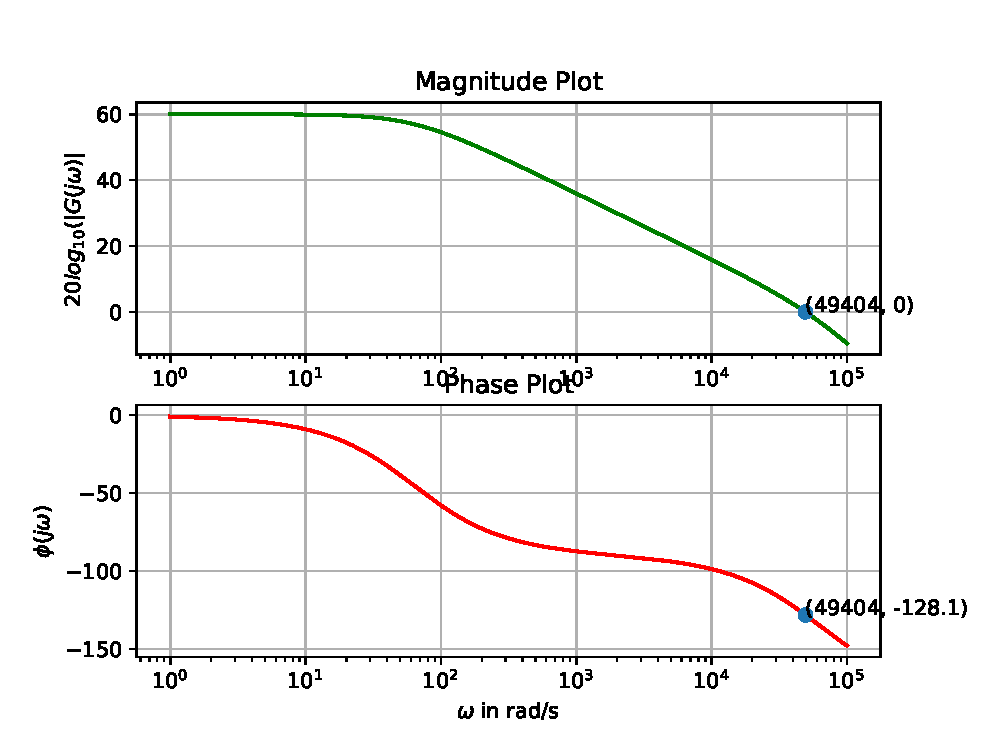
\includegraphics[width=\columnwidth]{./figs/ee18btech11034/ee18btech11034_1.eps}
\caption{}
\label{fig:ee18btech11034_1}
\end{figure}
%
\item Realise the above system with $PM = 51.9 \degree$ using a feedback circuit.
\item Find $H$ such that $PM = 45\degree$.
\\
\solution From \eqref{eq:ee18btech11034_phaseGH},
assuming constant $H$,
\begin{align}
\phase{G(f_{180})} = 45\degree - 180 \degree &=  -135\degree
\\
\implies -\tan^{-1}\brak{\frac{f}{10}} -\tan^{-1}\brak{\frac{f}{10^{4}}}  &= -135\degree
\\
\implies     \frac{\frac{f}{10} + \frac{f}{10^{4}}}{1-\frac{f^2}{10^{5}}} &= -1
\\
\text{or, }    f_{180} \approx 10 \, kHz
\end{align}
From \eqref{eq:ee18btech11034_1},
\begin{align}
\because  \abs{G\brak{f_{180}}H}&=1,
\\
  \frac{\brak{10^{5}}H}{\brak{\sqrt{1+\frac{10^{8}}{100}}}\brak{\sqrt{1+\frac{10^{8}}{10^{8}}}}} &= 1
\\
\implies     H &= 1.414 \times 10^{-2}
    \\
  \text{or, }  H_{max} =  1.414 \times 10^{-2}
\end{align}
which is the value of $H$ for which $PM > 45\degree$.

\item Verify the above using a Bode plot. 
\\
\solution 
The following code plots  Fig. \ref{fig:ee18btech11034_2}.
%
\begin{lstlisting}
codes/ee18btech11034/ee18btech11034_2.py
\end{lstlisting}
%
\begin{figure}[!h]
\centering
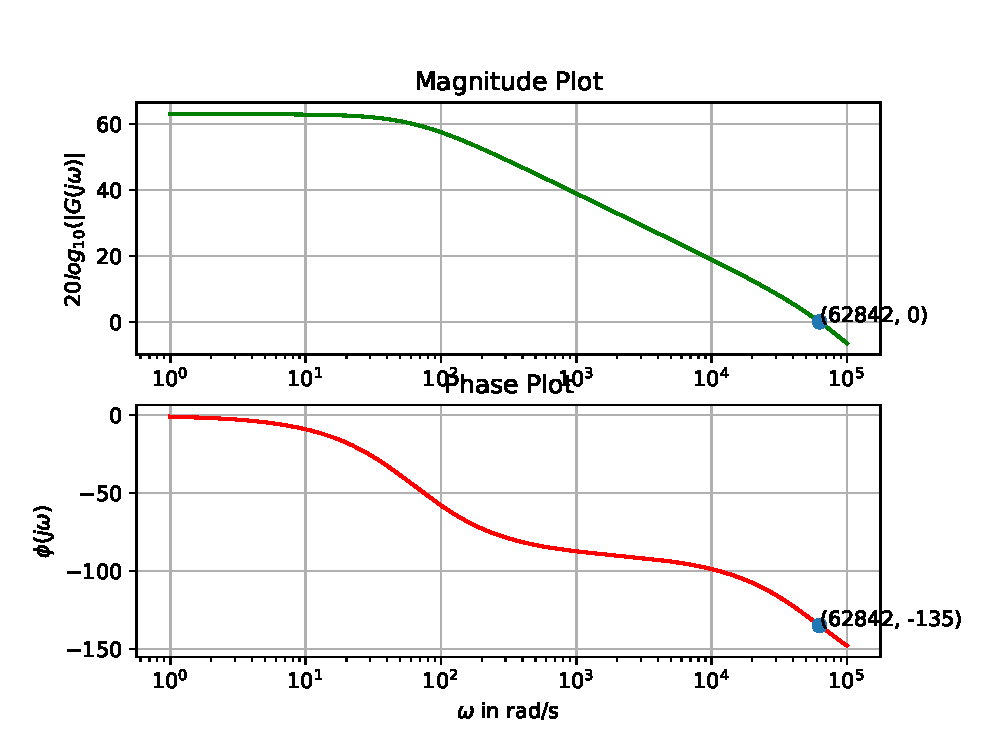
\includegraphics[width=\columnwidth]{./figs/ee18btech11034/ee18btech11034_2.eps}
\caption{}
\label{fig:ee18btech11034_2}
\end{figure}
\item Realise the above system with $PM = 45 \degree$ using a feedback circuit.

\end{enumerate}
